\documentclass[11pt]{article}

\usepackage[margin=1in]{geometry}
\usepackage[T1]{fontenc}
\usepackage{lmodern}
\usepackage{booktabs}
\usepackage{amsmath,amssymb}
\usepackage{graphicx}
\usepackage{enumitem}
\usepackage{microtype}
\usepackage[hidelinks]{hyperref}

\setlength{\parindent}{0pt}
\setlength{\parskip}{0.55em}
\setlist{nosep,leftmargin=*}

\title{How Many Measurements Does a Country Need\\Before Its IQB Score Is Reliable?}
\author{Interim Report}
\date{September 2026}

\begin{document}

\maketitle

\begin{abstract}
This interim report reviews an analysis of how many M-Lab measurements are needed to support a
country-level Internet Quality Barometer (IQB) score. The analysis uses 24 months of country-level
percentile aggregates, covering 245 countries and 5,720 country-months from January 2024 through
December 2025. The main result is a model-based planning requirement: at the p50 reporting level,
the smallest sample size is estimated so that the probability of being within $\pm 0.05$ IQB units
of a country's 24-month pooled target is at least 95\%. Under an independent-measurement model,
the median country requires approximately 560 download-side measurements, while the 90th-percentile
requirement is approximately 17,000. These values are lower bounds because M-Lab measurements are
clustered and the underlying network population changes over time. The report also evaluates
month-to-month score movement and the use of median absolute deviation (MAD), showing that MAD is
useful for describing observed volatility but is not an appropriate replacement for a tail-probability
criterion.
\end{abstract}

\section*{2. Project Summary}

This project evaluates whether the Internet Quality Barometer (IQB) provides a stable and policy-relevant
measure of Internet connectivity in countries with heterogeneous infrastructure. The broader research
examines four connected issues: sensitivity to percentile and threshold choices, the minimum number of
measurements needed for reliable scores, the usefulness of context-specific use-case profiles, and the
relationship between IQB results, urban--rural differences, market structure, and external socioeconomic
indicators.

The work completed to date focuses on the first phase of the proposal: robustness and thresholds. Using
24 months of M-Lab Network Diagnostic Tool aggregates, the analysis examines how IQB behaves when scores
are calculated at different percentile levels and when country sample sizes vary. A central finding is
that IQB can be reduced to ten weighted binary threshold tests. This makes it possible to estimate, for
each country and reporting level, the probability that finite-sample variation places the country on the
wrong side of an IQB threshold. Under an independent-measurement model, the median country requires
approximately 560 download-side measurements to be within $\pm0.05$ IQB units of its 24-month pooled
target with at least 95\% probability at p50. This is a planning lower bound rather than a guarantee for
a current month, because M-Lab measurements are clustered and network conditions change over time.

The interim outputs establish a quantitative basis for sample-size guidance and identify methodological
risks that must be addressed before using IQB as a policy classification tool. In particular, countries
close to hard IQB thresholds can remain unstable even with large samples, while a median absolute
deviation (MAD) of zero does not necessarily imply a reliable score. The next stages will extend this
work to context-specific use-case profiles, city-level and urban--rural comparisons, and validation
against external economic, infrastructure, and market indicators.

\section*{3. Progress Overview}

The original work plan divides the project into three phases of approximately two months each. Progress
against that plan is as follows:

\begin{table}[ht]
\centering
\caption{Progress against the proposed work plan.}
\begin{tabular}{p{0.20\linewidth}p{0.22\linewidth}p{0.48\linewidth}}
\toprule
Phase & Original focus & Progress \\
\midrule
1. Robustness and thresholds & Percentile sensitivity, sample-size requirements, and policy tipping points & Substantially advanced. The percentile structure, threshold crossings, sample-size requirements, bias, and key assumptions have been analysed. \\
2. Use-case profiles & Alternative weighting schemes and context-specific profiles & Not yet started as a dedicated analysis. The existing threshold decomposition provides the basis for this phase. \\
3. Urban--rural gap and external validation & City-level stability and correlations with external indicators & Not yet started. These remain planned next-period activities. \\
\bottomrule
\end{tabular}
\end{table}

The current work therefore addresses the sample-size component of Phase 1 in depth and provides a
methodological foundation for the remaining phases. The original proposal described bootstrap
resampling as the planned method. The completed analysis instead uses exact binomial and order-statistic
calculations, with Monte Carlo simulation used for validation. This change improves reproducibility and
avoids simulation error in the primary requirement estimates.

\section*{4. Key Achievements}

Major accomplishments to date include:
\begin{itemize}
  \item analysed 5,720 country-month observations covering 245 countries and 24 months of M-Lab data;
  \item verified that the IQB configuration reduces to ten distinct weighted threshold tests;
  \item derived a per-country, per-percentile sample-size requirement under an explicit 95\% criterion;
  \item quantified requirements for p50, p25/p50/p75, and all nine reported percentile levels;
  \item identified the effect of near-threshold countries, including cases that cannot be stabilized by
  additional samples under a hard-threshold scoring rule;
  \item measured the directional bias that can arise when under-sampled countries lose threshold tests;
  \item separated sampling error from observed month-to-month score movement;
  \item demonstrated that MAD is appropriate for descriptive volatility but not for a tail-probability
  reliability decision; and
  \item organized the work into reproducible notebooks, a methodological record, and generated output
  tables and figures.
\end{itemize}

\section*{5. Challenges and Mitigation Measures}

The main challenge has been that the available data are pre-aggregated to percentile knots rather than
retaining individual measurements. The analysis therefore reconstructs threshold pass rates from nine
percentiles. This is sufficient for aggregate planning estimates but introduces uncertainty for
individual countries, especially where packet loss has point masses or a threshold lies between sparse
percentile knots. The mitigation is to report aggregate medians and percentiles cautiously, identify
unresolved country-level cases, and recommend direct threshold pass counts in a future data pipeline.

A second challenge is dependence among measurements. Tests can be clustered by ASN, user, device, and
time of day, violating the independent-measurement assumption. The reported requirements are therefore
labelled lower bounds. The next analysis period will investigate whether ASN-, city-, or other cluster-
level aggregates can support an effective-sample-size or design-effect adjustment.

A third challenge is distinguishing sampling instability from real changes in connectivity and changes
in the population performing tests. The 24-month panel provides an empirical check, but it cannot fully
separate these mechanisms. The current mitigation is to treat the pooled result as a reference-target
planning estimate and to analyse observed temporal movement separately rather than presenting it as
sampling error.

\section*{6. Data and Methodology Update}

The current analysis uses M-Lab NDT country-level monthly aggregates from January 2024 through December
2025. Download and upload tables are joined by country and retain their separate sample counts. The IQB
calculation uses throughput, latency, and packet-loss percentiles at p1 through p99. The broader proposal
also identifies World Bank classifications, ITU broadband statistics, and ISP market data as future data
sources; these have not yet been incorporated into the current outputs.

The methodology differs from the original proposal in one important respect. Rather than relying on a
bootstrap over raw observations, the current analysis expresses IQB as ten threshold indicators and
uses exact binomial/order-statistic probabilities. This is appropriate for the step-valued IQB estimator
and avoids assuming that the four metric blocks are independently coupled at the individual-measurement
level. Monte Carlo resampling is retained as a validation tool. The primary target is the country's
24-month pooled distribution, evaluated at p50, with a tolerance of $\pm0.05$ and a 95\% probability
criterion. This target and criterion are explicit planning choices, not universal properties of IQB.

\section*{7. Deliverables to Date}

The following deliverables have been completed:
\begin{itemize}
  \item primary sample-size reliability notebook and per-country requirement table;
  \item score-volatility analysis using observed monthly IQB series;
  \item methodology review documenting assumptions, sensitivity checks, and limitations;
  \item focused evaluation of MAD as a reliability and volatility statistic;
  \item reader-facing explainer notebook describing the IQB threshold structure;
  \item written methodology document describing the estimator, criterion, verification, and limits; and
  \item generated CSV outputs and figures for sample-size, volatility, methodology-review, and MAD
  diagnostics.
\end{itemize}

No external-data validation, alternative use-case profile, city-level analysis, or urban--rural
comparison has yet been delivered. These are part of the remaining work plan.

\section*{8. Work Plan for Next Period}

The next period will extend the completed Phase 1 foundation and begin the remaining proposal phases:
\begin{enumerate}
  \item refine the sample-size analysis using cluster-level information where available and quantify
  effective sample sizes;
  \item analyse country-level versus city-level IQB stability to investigate whether national scores
  mask urban--rural differences;
  \item integrate World Bank income classifications and relevant infrastructure indicators to test
  whether threshold sensitivity differs by development context;
  \item design alternative use-case weighting profiles, including a profile that de-emphasizes use
  cases such as gaming where justified by the research context;
  \item obtain and harmonize ITU broadband and ISP market-concentration indicators, including HHI where
  data coverage permits;
  \item compare default and context-specific IQB scores using rank correlations and threshold-crossing
  counts; and
  \item prepare updated technical documentation, figures, and a draft conference or final report.
\end{enumerate}

The proposed sequencing is to complete the cluster and city-level data assessment first, then conduct
the contextual profile and external-validation analyses. Results will be recorded in the existing
notebook workflow so that the sample-size, sensitivity, and validation analyses remain reproducible.

\section*{9. Support Required}

The immediate support required is methodological and data-oriented. Assistance from ISOC or project
partners would be valuable in confirming whether $\pm0.05$ and 95\% are appropriate publication criteria,
identifying the intended policy interpretation of minimum and high-quality thresholds, and reviewing
which use cases should receive different weights in different development contexts.

Access to more detailed M-Lab aggregates would substantially improve the next phase. In particular,
ASN-, city-, device-, or user-level counts and direct threshold pass counts would support dependence
adjustment and reduce uncertainty from percentile reconstruction. Guidance on authoritative sources for
ISP market concentration, ITU indicators, and country development classifications would also reduce
data-integration risk. No additional computational infrastructure is currently required for the
existing analysis.

\section*{10. Expected Impact}

The expected impact is a more transparent and defensible use of IQB in country reports and policy
analysis. The completed work shows that a country-level score should not be interpreted solely from its
point estimate. Its reliability depends on sample size, distance from hard thresholds, reporting
percentile, and the target period. Making these dependencies explicit can prevent sparse or
near-threshold countries from being ranked or classified with unjustified precision.

The next phases will assess whether methodological sensitivity is systematically related to development
context, urban--rural structure, or market concentration. This can reveal whether aggregate IQB scores
hide connectivity disadvantages or produce apparently stable results because of measurement composition.
Alternative use-case profiles may also make the metric more relevant to distinct policy objectives,
provided that the profiles are documented and evaluated rather than introduced informally.

In technical terms, the project will provide a framework for attaching uncertainty, sensitivity, and
context to IQB scores. In policy terms, it can support more accountable decisions about infrastructure
investment, funding eligibility, and regulatory classification by distinguishing observed network
quality from artefacts of sampling and methodological choice.

\section{Research Question and Scope}

The project asks: \emph{how many measurements are needed per country before an IQB computation can
be treated as reliable?} This question has two distinct components. First, a finite sample can place
a country on the wrong side of one or more IQB thresholds. This is sampling error and can, in
principle, be reduced by collecting more measurements. Second, a country's measured network
conditions can genuinely change between months, and the population performing M-Lab tests can also
change. This temporal and population variation is not removed simply by increasing the number of
tests in one month.

The primary analysis therefore uses a precise, limited definition of reliability. For a selected
country and reporting percentile, the requirement is the smallest sample size $n$ satisfying
\begin{equation}
  \Pr\left(\left|\widehat{\mathrm{IQB}}_n-
  \mathrm{IQB}_{\mathrm{target}}\right| \leq 0.05\right) \geq 0.95.
\end{equation}
The target is the country's 24-month pooled distribution, evaluated at p50 unless otherwise
specified. This is appropriate for capacity planning against a stable reference distribution,
but it is not a guarantee that a score for one current month represents the current month's
underlying network conditions.

The analysis deliberately separates this primary criterion from two descriptive questions. The
first is how much IQB varies across the observed 24-month history. The second is whether MAD is a
useful summary of that variation. These diagnostics provide context for interpreting the sample-size
calculation, but they do not replace the 95\% probability criterion.

\section{Data and Analytical Materials}

The input consists of monthly country-level M-Lab aggregates stored in the project data directory.
Each country-month contains sample counts and nine percentile knots: p1, p5, p10, p25, p50, p75,
p90, p95, and p99. The panel contains 5,720 country-month rows from 245 countries over 24 months.
The median number of download-side measurements per country-month is approximately 4,801; the
10th percentile is approximately 90 and the 90th percentile is approximately 548,317.

The data are separated into download and upload tables. Latency and packet-loss tests are measured
on the download side, while upload-throughput tests use upload-side measurements. Consequently,
there is not one universally correct sample count for every IQB component. The main requirement is
reported in download-side measurements and accounts for each country's upload-to-download ratio
when evaluating upload thresholds.

The work is organized into five surviving notebooks. Notebook 03 is the primary sample-size
calculation. Notebook 04 measures observed month-to-month IQB volatility. Notebook 05 reviews the
assumptions and sensitivity of the method. Notebook 06 evaluates MAD as a reliability statistic.
Notebook 07 explains the estimator and results for readers who do not need every implementation
detail. Notebooks 01 and 02 provide earlier setup and CDF work and are outside the scope of this
interim report.

\section{IQB as a Threshold Estimator}

IQB is implemented as weighted averages of use-case scores and network-requirement scores. Each
network requirement is binary: a metric either passes or fails a fixed threshold. Although the
configuration contains 24 use-case-by-requirement combinations, repeated requirements ask the same
question. Flattening the weights produces ten distinct metric-threshold tests:

\begin{table}[ht]
\centering
\caption{The ten distinct IQB threshold tests and their combined weights.}
\label{tab:tests}
\begin{tabular}{lrlr}
\toprule
Test & Weight & Test & Weight \\
\midrule
loss $<0.01$ & 0.2021 & upload $>25$ & 0.1285 \\
latency $<100$ & 0.1644 & loss $<0.005$ & 0.0809 \\
download $>10$ & 0.1416 & upload $>10$ & 0.0495 \\
download $>25$ & 0.1285 & latency $<10$ & 0.0490 \\
 & & latency $<50$ & 0.0417 \\
 & & upload $>5$ & 0.0139 \\
\bottomrule
\end{tabular}
\end{table}

\begin{figure}[htbp]
\centering
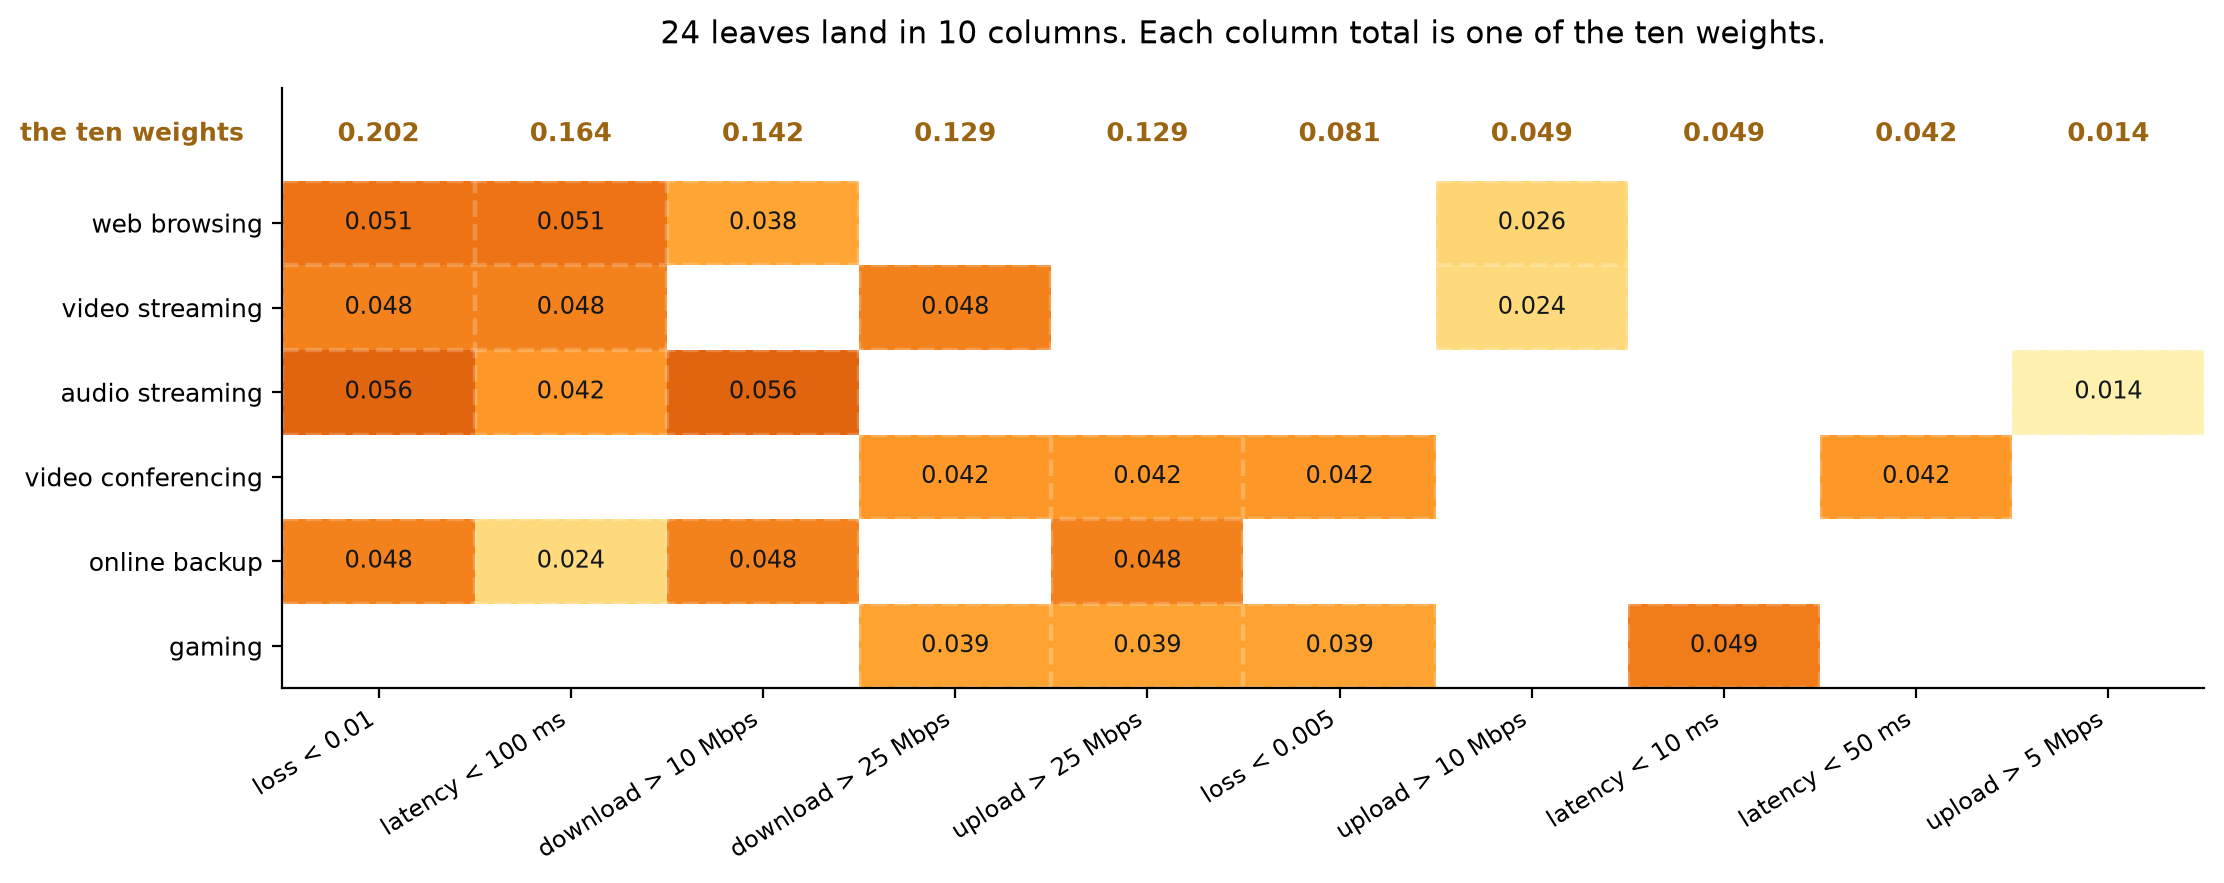
\includegraphics[width=0.98\linewidth]{analysis_outputs/explainer_figures/fig1_the_collapse.png}
\caption{The 24 use-case-by-requirement leaves collapse into ten distinct weighted threshold tests.
Repeated thresholds are not independent questions: they contribute to the same IQB component.}
\label{fig:collapse}
\end{figure}

If $I_k$ indicates whether threshold test $k$ passes and $w_k$ is its combined weight, then
\begin{equation}
  \mathrm{IQB}=\sum_{k=1}^{10}w_k I_k, \qquad \sum_{k=1}^{10}w_k=1.
\end{equation}
This reduction is important because IQB is not a smooth average of measurements. The score changes
only when a percentile crosses a threshold. A sampling error that does not cross a threshold has no
effect on the score; a single crossing can cause a relatively large jump. Six of the ten tests have
individual weights greater than 0.05, so one incorrectly classified test can by itself exceed the
chosen tolerance.

For reporting percentile $q$, a threshold pass can be expressed as a question about a pass rate.
Let $\pi_k$ be the fraction of measurements that pass threshold $k$. The corresponding quantile
passes when
\begin{equation}
  q > 1-\pi_k.
\end{equation}
Thus each IQB test becomes a binomial classification problem: the observed pass count must be on
the correct side of a percentile-dependent cutoff.

\section{Sample-Size Method}

For intuition, suppose measurements are independent and each passes a fixed threshold with
probability $\pi$. The pass count has distribution $X\sim\mathrm{Binomial}(n,\pi)$ and standard
deviation $\sqrt{n\pi(1-\pi)}$. The distance from the expected count to the decision cutoff is
$\delta n$, where $\delta=|\pi-(1-q)|$. The usual normal approximation gives
\begin{equation}
  n \gtrsim \frac{\pi(1-\pi)z^2}{\delta^2},
\end{equation}
where $z$ is the normal critical value associated with the desired probability.

The implemented calculation uses an exact order-statistic formulation rather than relying on this
approximation at small sample sizes. For $n$ independent observations, the sample $q$-quantile is
the $r$th order statistic, with $r=\lceil qn\rceil$. Its position on the underlying CDF follows
\begin{equation}
  U=F(\widehat Q_q)\sim\mathrm{Beta}(r,n-r+1).
\end{equation}
The probability that each threshold is classified correctly can therefore be evaluated from exact
binomial or beta tails. The full IQB sampling distribution is obtained by combining the nested
thresholds within each metric and then summing the weighted threshold indicators.

The pass rates are not directly available in the aggregates. They are reconstructed from the nine
reported percentile knots after mapping each metric into a quality scale where larger values are
better. Throughput is transformed logarithmically, latency is reversed, and loss is handled with a
linear reversal because it has a substantial point mass at zero. The reconstruction is a necessary
approximation and is one of the main sources of uncertainty for individual countries.

The target distribution is formed over the 24-month panel. Pooling is performed in threshold space:
the pass rate at a fixed threshold is a sample-weighted average of monthly pass rates. This is valid
for a CDF evaluated at a fixed value, unlike averaging monthly quantiles. The resulting requirement
is therefore a requirement for matching the pooled reference distribution, not a requirement for
auditing a single month.

\section{Results}

Table~\ref{tab:requirements} summarizes the main output. At p50 and a tolerance of $\pm0.05$ with
95\% probability, the median country requires approximately 560 download-side measurements. The
90th-percentile requirement is approximately 17,000. The requirement is highly heterogeneous:
countries close to a threshold can require orders of magnitude more measurements than countries
with a comfortable margin, and countries exactly on a threshold cannot be stabilized by additional
measurements under this scoring rule.

\begin{table}[ht]
\centering
\caption{Model-based requirements for the pooled reference distribution.}
\label{tab:requirements}
\begin{tabular}{lrrr}
\toprule
Publication target & Median requirement & 90th percentile & Sufficient today \\
\midrule
p50 alone & $\sim$560 & $\sim$17,000 & 185 / 245 \\
p25, p50, p75 & $\sim$2,400 & $\sim$86,000 & 138 / 245 \\
all nine levels & $\sim$5,400 & $\sim$114,000 & 111 / 245 \\
\bottomrule
\end{tabular}
\end{table}

The all-nine requirement is substantially larger because every reporting level introduces a
different cutoff. A country that is safely measured at p50 can still be close to a threshold at p75
or p90. This is why a single global sample-size rule is not appropriate when the full percentile
curve is published.

Figure~\ref{fig:margin} illustrates the main driver of this variation. Required sample size grows
rapidly as the pass rate approaches a consequential cutoff. The horizontal axis is the distance from
the nearest cutoff in pass-rate space, rather than a country-size or population measure.

\begin{figure}[htbp]
\centering
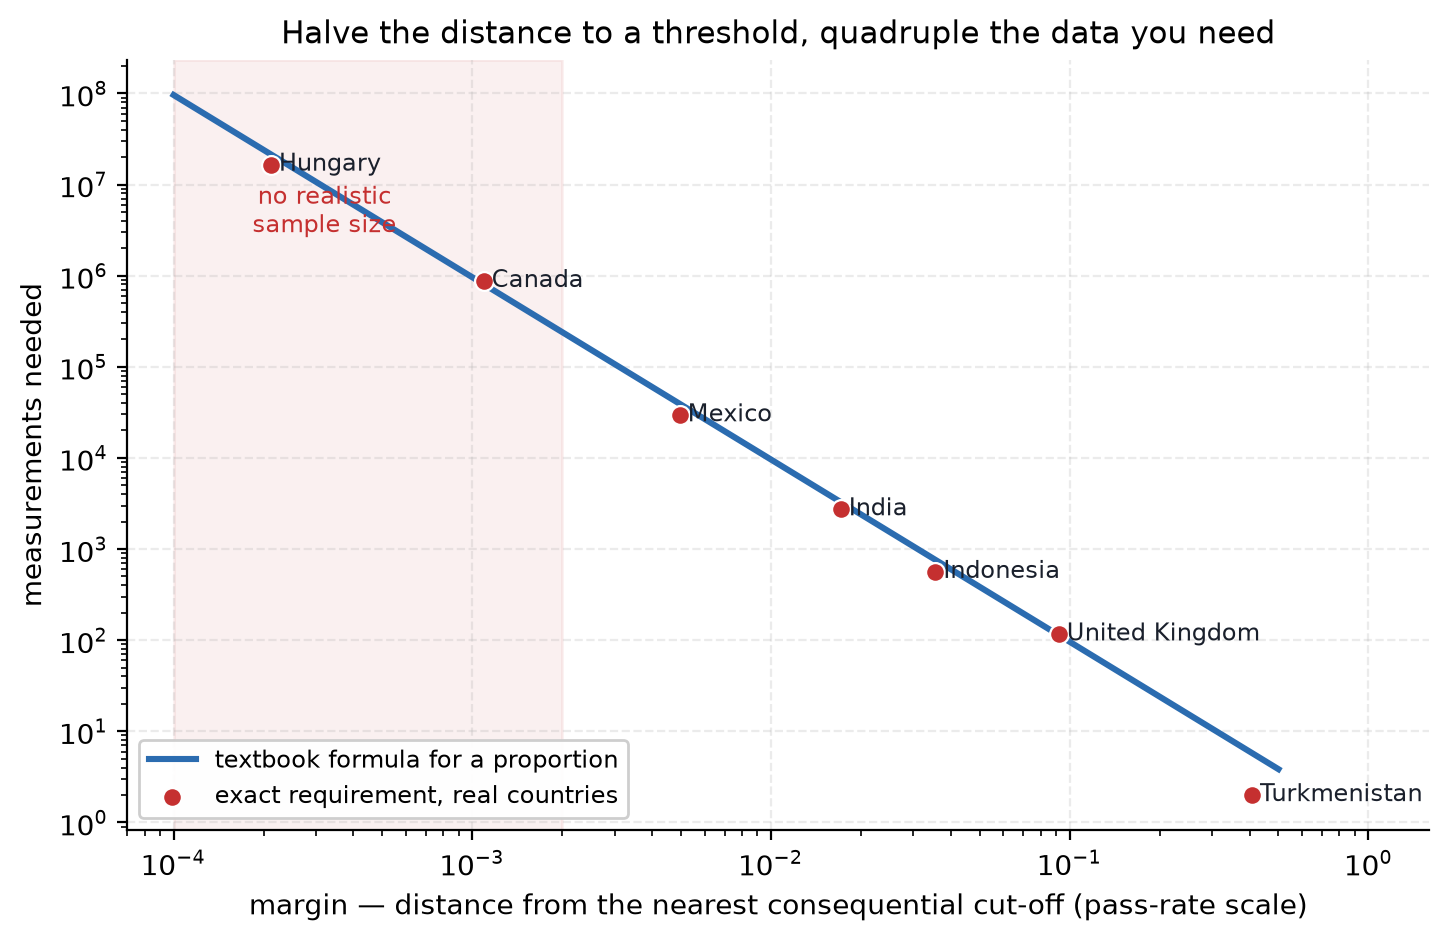
\includegraphics[width=0.92\linewidth]{analysis_outputs/review_figures/fig2_margin_to_sample_size.png}
\caption{Required measurements increase sharply as a country's pass rate approaches an IQB cutoff.
The plotted country examples show why a universal sample-size rule is inappropriate.}
\label{fig:margin}
\end{figure}

The analysis also identifies a directional bias for under-sampled countries. Because IQB is a sum of
binary tests, a country near a high score can lose points when a threshold is incorrectly classified,
without an equivalent upward movement in the observed estimate. In the current output, 24 of 245
countries have estimated bias larger than the $\pm0.05$ tolerance, with the largest reported bias
approximately $-0.33$. This reinforces the need to treat small-sample scores as potentially biased,
not merely noisy.

\section{Observed Volatility and the Role of MAD}

Notebook 04 evaluates the observed IQB series over the 24-month panel at p50 and p90. Its purpose is
different from the primary sample-size calculation: it asks how much a country's score actually
moved, rather than how much a fixed target score would move under repeated independent sampling.
The typical monthly sample count varies widely, so the analysis compares country-level sample counts
with the median absolute deviation of the observed monthly score series.

MAD is defined as
\begin{equation}
  \mathrm{MAD}=\mathrm{median}\left(|x_i-\mathrm{median}(x)|\right).
\end{equation}
It is robust to occasional jumps and is therefore useful for describing the typical state of a
country over time. However, notebook 06 shows why MAD is not an appropriate confidence criterion
for the sampling problem. IQB is discrete. If the most probable score has probability greater than
one half, the median and the middle half of the sampling distribution can lie at the same point,
making MAD exactly zero even when a substantial minority of resamples produce an IQB error larger
than 0.05.

In one diagnostic at $n=100$, the median country has MAD equal to zero while approximately 29\% of
resamples are more than 0.05 IQB units from the target. At $n=1{,}000$, the median MAD remains zero
while the median probability of obtaining the exact target is approximately 96\%. These results do
not make MAD useless. They show that MAD answers a middle-of-distribution question, whereas the
sample-size requirement is a tail-probability question. The report therefore uses the exact
probability criterion for planning and MAD only for descriptive temporal volatility.

Figure~\ref{fig:mad} shows this distinction directly: MAD remains at zero while the standard
deviation and mean absolute error respond to the probability mass moving across the threshold.

\begin{figure}[htbp]
\centering
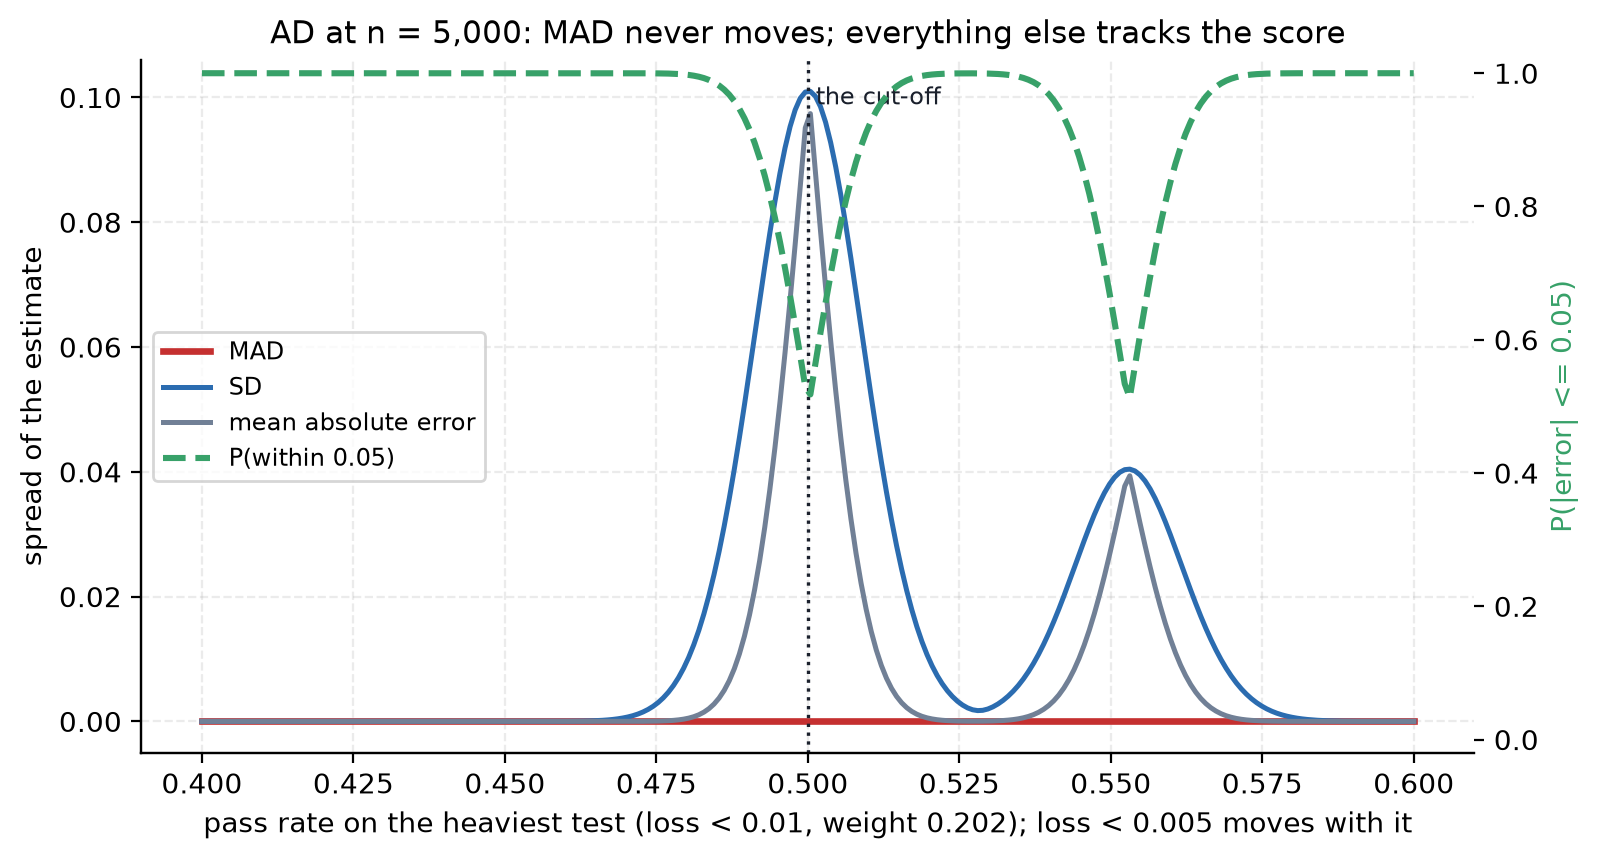
\includegraphics[width=0.96\linewidth]{analysis_outputs/mad_figures/fig5_mad_does_not_respond.png}
\caption{At $n=5{,}000$, MAD remains zero across a range of pass rates even though other error
measures and the probability of being within the tolerance change. This is why MAD is descriptive
rather than a decision rule for sample-size sufficiency.}
\label{fig:mad}
\end{figure}

\section{Validation and Limitations}

Several parts of the analysis were checked independently. The ten-test decomposition agrees with
the production \texttt{IQBCalculator} to floating-point precision across sampled country-percentile
pairs. The exact sampling distribution agrees with Monte Carlo simulation when both use the same
reconstructed probability model. The nested threshold structure is preserved across the metrics,
and the implied IQB score is non-decreasing as the reporting percentile increases.

The most important limitations are methodological rather than computational:
\begin{enumerate}
  \item \textbf{Independence.} M-Lab measurements cluster by ASN, user, device, and time of day.
  The independent-measurement requirement is therefore a lower bound. The current aggregates do
  not provide enough information to estimate an effective sample size or design effect reliably.
  \item \textbf{Changing target.} The 24-month pooled target is useful for planning but may not
  represent the current month. Month-to-month movement includes real network change and changes in
  who performs tests.
  \item \textbf{Percentile reconstruction.} Only nine percentile knots are available. Thresholds
  between knots require interpolation, and packet loss has point masses that make tie handling
  consequential. Per-country requirements are less certain than aggregate medians and percentiles.
  \item \textbf{Current-month confidence.} The existing data cannot support a cluster-adjusted
  guarantee for a current-month IQB score. That question requires more detailed measurement-level
  or cluster-level information.
  \item \textbf{Policy choice.} The $\pm0.05$ tolerance and 95\% probability level are explicit
  planning choices, not properties of IQB itself. Different publication goals require recomputing
  the requirement.
\end{enumerate}

\section{Interim Conclusions and Next Steps}

The completed work establishes a defensible first answer to the sample-size question, provided the
scope is stated correctly. There is no universal number of measurements per country. The requirement
depends on the reporting percentile, the country's distance from IQB thresholds, and whether the
target is a pooled distribution or a current month. For the pooled p50 target, the median iid
planning requirement is about 560 download-side measurements for $\pm0.05$ accuracy at 95\%
probability; this should be interpreted as a lower bound, not as a production guarantee.

The next stage should focus on reducing the gap between this lower-bound planning result and an
operational reporting rule. Priority tasks are:
\begin{enumerate}
  \item obtain or derive ASN-, city-, device-, or user-level information sufficient to estimate
  effective sample sizes;
  \item repeat the analysis for an explicitly current-month target rather than only the pooled
  24-month target;
  \item replace percentile-knot reconstruction with direct threshold pass counts if the aggregation
  pipeline can be extended;
  \item decide whether IQB should publish a point estimate, an uncertainty band, or suppress scores
  that are unresolved because they lie close to a threshold; and
  \item confirm with stakeholders whether $\pm0.05$ and 95\% are the appropriate publication bar.
\end{enumerate}

\section*{Reproducibility}

The analysis is implemented in the notebooks \texttt{03-sample\_size\_reliability.ipynb} through
\texttt{07-explainer.ipynb}. The primary per-country output is
\texttt{analysis\_outputs/03\_sample\_size\_requirements.csv}. The written methodological record
is \texttt{METHODOLOGY.md}. The notebooks use the project data under \texttt{data/v1/}; rerunning
the primary analysis regenerates the requirement table.

\end{document}